In this section, we introduce a notion of weighted type graphs which modifies the notion presented in \cite{endrullis2024generalized}.

\begin{definition}[Weighted Type Graph]
    \label{def:weighted_type_graph}
    A \textbf{weighted type graph} \(\mathcal{T} \mathop{=} (T, \mathbb{E}, \mathcal{S}, w)\) consists of:
    \begin{itemize}
        \item A \textbf{type graph} \(T\),
        \item A set \(\mathbb{E}\) of \textbf{\(T\)-valued elements} \(e \mathop{\in} \mathcal{C}_1\) with $\operatorname{codom}(e) \mathop{=} T$,
        \item A strongly monotonic measurable semiring \(\mathcal{S}=(S, \mathop{\oplus}, \mathop{\odot}, 0_S, 1_S, \prec, \mu)\),
        \item A weight function \(w : \mathbb{E} \mathop{\to} S \mathop{\setminus} \{0_S\}\) such that \(w(e) \mathop{\neq} 0_S\) for all \(e \mathop{\in} \mathbb{E}\).
    \end{itemize}
    \(\mathcal{T}\) is \textbf{finitary} if for every \((e:X \mathop{\to} T) \mathop{\in} \mathbb{E}\) and \(G \mathop{\in} \mathcal{C}_0\), \(\operatorname{Hom}(X, G)\) and \(\operatorname{Hom}(G, T)\) are finite sets.
\end{definition}

\begin{remark}
    \label{remark:greater_than_1}
    Our definition removes the requirement \(w(e) \mathop{\succeq} 1_S\) present in the type graph definition of~\cite{endrullis2024generalized}. While this condition is used in Lemma~4.10(b) of prior work to ensure \(a \mathop{\odot} b \mathop{\succeq} a\) when \(b \mathop{\neq} 0_S\), it is not fundamental to the type graph method itself. Specifically, for DPO rewriting systems that only modify edge labels and preserve graph structure, this condition is unnecessary.
\end{remark}

\begin{remark}
    \label{remark:semiring_0_unpredictable}
    The requirement \(\forall e \mathop{\in} \mathbb{E}, w(e) \mathop{\neq} 0_S\) is necessary because \(0_S\) behaves unpredictably in strongly monotonic measurable semirings. For instance, in the natural and real tropical semirings \((\mathbb{N} \mathop{\cup} \{\mathop{+\infty}\}, \mathop{\min}, +)\), \(0_S\) is the greatest element \(\mathop{+\infty}\), while in the natural and real arctic semirings \((\mathbb{N} \mathop{\cup} \{\mathop{-\infty}\}, \max, +)\), \(0_S\) is the smallest element \(\mathop{-\infty}\).
\end{remark}

\section{Weighing Morphisms and Objects} 
\label{sec:weigh_morphisms_and_objects}
In this section, we explain how the type graph method assigns weights to both morphisms targeting the type graph and to objects.
\begin{notation}[\cite{endrullis2024generalized}] For morphisms \( \alpha : A \mathop{\to} B \), \( \beta : B \mathop{\to} C \), \( \gamma : A \mathop{\to} C \) and $E \mathop{\subseteq} \operatorname{Hom}(A,B)$, define:
 \begin{flalign*}
            \set{ \alpha \mathop{\star} - \mathop{=} \gamma } &\overset{\operatorname{def}}{=} \{ \beta \mathop{\in} \operatorname{Hom}(B, C) \mid \alpha \mathop{\star} \beta \mathop{=} \gamma \}.
\\
            \set{ - \mathop{\star} \beta \mathop{=} \gamma }  &\overset{\operatorname{def}}{=} \{ \alpha \mathop{\in} \operatorname{Hom}(A, B) \mid \alpha \mathop{\star} \beta \mathop{=} \gamma \}.
\\
            E \mathop{\star} \beta                   &\overset{\operatorname{def}}{=} \set{ \alpha \mathop{\star} \beta \mid \alpha \mathop{\in} E }.
 \end{flalign*}
\end{notation} 

\begin{definition} 
    \label{def:bigodot}
Let $(S, \mathop{\oplus}, \mathop{\odot}, 0_s, 1_s)$ be a semiring. We define 
 \begin{flalign*}
    \mathop{\bigodot} \emptyset &\overset{\operatorname{def}}{=} 1_s
\\
    \mathop{\bigodot} \left( E \mathop{\cup} \{x\} \right) &\overset{\operatorname{def}}{=} \left( \mathop{\bigodot} E \right) \mathop{\odot} x
    \\
    \mathop{\bigoplus} \emptyset &\overset{\operatorname{def}}{=} 0_s
    \\
        \mathop{\bigoplus} \left( E \mathop{\cup} \{x\} \right) &\overset{\operatorname{def}}{=} \left( \mathop{\bigoplus} E \right) \mathop{\oplus} x
\end{flalign*}
\end{definition}


\begin{definition}[Morphism weight \cite{endrullis2024generalized}]
    \label{def:weight}
    Let $\mathcal{T} \mathop{=} (T,\mathbb{E},S, w)$ be a finitary type graph.
    \newline
    \noindent
    \begin{minipage}{0.6\textwidth}
        The \textbf{weight of a morphism $h: G \mathop{\rightarrow} T$ relative to $(e:X \mathop{\to} T) \mathop{\in} \mathbb{E}$} is defined as the weight $w(e)$ raised to the power of the number of $\iota$ making the diagram (shown on the right) commutative.
    \end{minipage}
    \begin{minipage}{0.29\textwidth}
        \begin{center}
                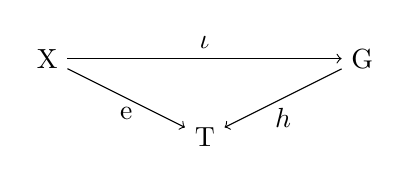
\begin{tikzpicture}
                    \node (a) at (0,0) {X};
                    \node (c) at (4,0) {G};
                    \node (d) at (2,-1) {T};
                    \draw[->] (a) -- (d) node [midway,below] {e};
                    \draw[->] (a) -- (c) node [midway,above] {$\iota$};
                    \draw[->] (c) -- (d) node[midway, below] {$h$};
                    % \node (d) at (2,-0.5) {=};
                \end{tikzpicture}
        \end{center} 
    \end{minipage}
                \[
                w_e(h) 
                    \overset{\operatorname{def}}{=}
                \underset{\alpha \mathop{\in} \{- \mathop{\star} h \mathop{=} e\}}{\mathop{\bigodot}}w(e) 
                \]
        % which can be visualized as $w(e)$ raised to the power of the number of possible morphisms $g$ which make the following commutative diagram hold

        \noindent
        The \textbf{weight of a morphism $h: G \mathop{\rightarrow} T$ relative to \(\mathcal{T}\)} is defined as the semiring product of $w(e)$ for $e \mathop{\in} \mathbb{E}$:
        \[  w_\mathcal{T}(h) \overset{\operatorname{def}}{=} \underset{e \mathop{\in} \mathbb{E}}{\mathop{\bigodot}} 
                w_e(h) \]

        \noindent
       The \textbf{weight of an object \( G \mathop{\in} \mathcal{C}_0 \) relative to \( \mathcal{T}\)} is defined as the semiring sum of $w_\mathcal{T}(h)$ for $h \mathop{\in} \operatorname{Hom}(G,T)$:
        \[w_\mathcal{T}(G) \overset{\operatorname{def}}{=} \underset{h \mathop{\in} \operatorname{Hom}(G,T)}{\mathop{\bigoplus}}  w_\mathcal{T}(h) \]
\end{definition}


% In certain scenarios, we want to exclude specific morphisms when calculating morphism weight relative to a give T-valued element $e:X \mathop{\to} T$. For this reason, for all set \( \Gamma \mathop{\subseteq} \operatorname{Hom}(A, G) \), we define 



% The weight of the morphism \( \phi : G \mathop{\to} T\) excluding morphisms in \( \Gamma' \) is defined as the number of morphisms from \( X \) to \( G \) that do not factor through any \( \alpha \mathop{\in} \Gamma \).

\begin{definition}[Weight excluding specific morphisms \cite{endrullis2024generalized}]
    \label{def:weight_excluding}
    Let \( A \mathop{\in} \mathcal{C}_0 \) and $\Gamma \mathop{\subseteq} \operatorname{Hom}(A,G)$.
    \newline
    \noindent
    \begin{minipage}{0.6\textwidth}
        We define $\Gamma'$ as the set consisting of all morphisms \( \iota : X \mathop{\to} G \) admitting morphisms \( \zeta \mathop{\colon} X \mathop{\to} A \) and \( \alpha \mathop{\in} \Gamma \) such that the diagram illustrated on the right is commutative. Formally, 
    \end{minipage}
    \begin{minipage}{0.4\textwidth}
        \hfill 
        % \begin{center}
            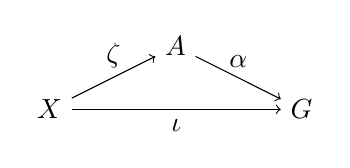
\begin{tikzpicture}[scale=0.8]
                \node (X) at (0,0) {\(X \)};
                \node (A) at (2,1) {\( A \)};
                \node (G) at (4,0) {\( G \)}; 
                \draw[->] (X) -- (A) node[midway, above] {\( \zeta \)};
                \draw[ ->] (X) -- (G) node[midway, below] {\( \iota \)};
                \draw[->] (A) -- (G) node[midway, above] {\( \alpha \)};
                % \node at (2,0.5) {\( \mathop{=} \)};
                % \node (T) at (2,-1) {\( T \)};
                % \draw[ ->] (X) -- (T) node[midway, below] {e};
                % \draw[<-] (T) -- (G) node[midway, above] {};
            \end{tikzpicture}
        % \end{center} 
    \end{minipage}

    \[
    \Gamma' \overset{\operatorname{def}}{=} \left\{ \iota \mathop{\in} \operatorname{Hom}(X, G)~\middle|~\exists \alpha \mathop{\in} \Gamma,~\exists \zeta:X \mathop{\to} A,~\zeta \mathop{\star} \alpha \mathop{=} \iota \right\}.
    \]

    \noindent
    The \textbf{weight of a morphism \(h : G \mathop{\to} T\) excluding morphisms in \( \Gamma' \) relative to $(e:X \mathop{\to} T) \mathop{\in} \mathbb{E}$} is defined as $w(e)$ raised to the power of the number of morphisms \( (\iota : X \mathop{\to} G) \notin \Gamma' \).
        \[
        w_e(h - \Gamma) \overset{\operatorname{def}}{=} \underset{
            \substack{\alpha \mathop{\in} \set{- \mathop{\star} h \mathop{=} e} \\
                        \alpha \notin \Gamma'}}{\mathop{\bigodot}} w(e)\] 
        The \textbf{weight of a morphism $h: G \mathop{\to} T$ excluding morphisms in \( \Gamma' \) relative to \(\mathcal{T}\)} is defined as the semiring product of $w_e(h-\Gamma)$ for $e \mathop{\in} \mathbb{E}$:
        \[ 
            w_\mathcal{T}(h-\Gamma) \overset{\operatorname{def}}{=} \underset{e \mathop{\in} \mathbb{E}}{\mathop{\bigodot}} 
        w_e(h-\Gamma)
                \]
\end{definition} 
% \begin{definition}[Weight excluding morphisms \cite{endrullis2024generalized}]
%     \label{def:weight_excluding}
%     Let \(\Gamma \mathop{\subseteq} \operatorname{Hom}(A, G)\). Define:
%     \[
%     \Gamma' \overset{\text{def}}{=} \left\{ \iota \mathop{\in} \operatorname{Hom}(X, G) \,\middle|\, \exists \alpha \mathop{\in} \Gamma, \exists \zeta : X \mathop{\to} A, \, \zeta \mathop{\star} \alpha \mathop{=} \iota \right\}.
%     \]
%     The \textbf{weight of \(h : G \mathop{\to} T\) excluding \(\Gamma'\)} is:
%     \[
%     w_e(h - \Gamma) \overset{\text{def}}{=} \mathop{\bigodot}_{\substack{\iota \mathop{\in} \{- \mathop{\star} h \mathop{=} e\} \\ \iota \notin \Gamma'}} w(e), \quad
%     w_\mathcal{T}(h - \Gamma) \overset{\text{def}}{=} \mathop{\bigodot}_{e \mathop{\in} \mathbb{E}} w_e(h - \Gamma).
%     \]
% \end{definition}
    If \( \Gamma \) is a singleton \( \{ \alpha \} \), we denote \( w_{\mathcal{T}_\Sigma^X}(h - \alpha) \) instead of \( w_{\mathcal{T}_\Sigma^X}(h - \{ \alpha \}) \).
